% \chapter{Introduction \Author{J. Singer}\\\progressbar[0.4\textwidth]{draft}{70}}
\chapter{Introduction \Author{J. Singer}}
\inputprogress
\label{chapter:vanilla}

\inputpath{part1}{vanilla}

%%%%%%%%%%%

% Possibility of unique names for distinct entities.
% Maybe a slightly humorous example, involving Homer Simpson and
% Homer the classical Greek poet. Convey the point that,
% without unique names, extra \textit{context} is required
% to make the name useful.
% (Springfield or Greece?)

In computer programming, as in real life, 
names are useful handles for concrete entities.
% Discuss the utility of names as abstract identifiers.
The key message of this book is that
having \textit{unique names} for
\textit{distinct entities}
reduces uncertainty and imprecision.

For example, consider overhearing a conversation
about `Homer.' Without any more contextual clues, you
cannot disambiguate between Homer Simpson and Homer the
classical Greek poet; or indeed, any other people
called Homer that you may know.
As soon as the conversation mentions Springfield
(rather than Smyrna), you are fairly sure that the
Simpsons television series (rather than Greek poetry)
is the subject.
On the other hand, if everyone had a \textit{unique} name,
then there would be no possibility of confusing 20th century
American cartoon characters with ancient Greek literary figures.

%% \todo{Are we allowed to have a cartoon picture such as this one here?}
%% \begin{center}
  %% 
\includegraphics[width=.3\textwidth]{homer-simpson}
  %% \qquad
  %% \raisebox{2cm}{\Huge $\neq$}
  %% \qquad
  %% 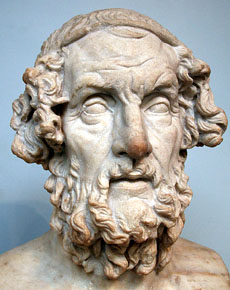
\includegraphics[width=.3\textwidth]{homer-poet}
%% \end{center}


% where SSA is applied, in compiler intermediate representations...
This book is about the \textit{static single assignment form} (SSA),
which is a naming convention for storage locations (variables)
in low-level representations
of computer programs.
%% remove following definition, since we have a full Section
%% on definition coming up soon...
% A program is said to be in SSA form when each variable is defined (hence
% \textit{assignment})
% exactly once (hence \textit{single}) in the program text
% (hence \textit{static}).
The term \textit{static} indicates that SSA relates to properties
and analysis of program text (code).
% that occurs inside a 
% compiler, prior to execution.
The term \textit{single} refers to the uniqueness property of
variable names that SSA imposes. As illustrated above, this enables
a greater degree of precision.
The term \textit{assignment} means variable definitions. For
instance, in the code
\begin{equation*}
\begin{array}{l}
x = y+1;
\end{array}
\end{equation*}
the variable $x$ is being assigned the value of expression $(y+1)$.
This is a definition, or assignment statement, for $x$.
A compiler engineer would interpret the above assignment statement
to mean that the lvalue of
$x$ (i.e., the memory location labelled as $x$) should be modified to store
the value $(y+1)$.

%%%%%%%%%%%%%%%%%%%%%

\section{Definition of SSA}


The simplest, 
least constrained, definition of SSA can be given using the following informal prose:
%% \index{SSA, informal definition of}

\begin{quote}
A program is defined to be in SSA
form if each variable is a target of
exactly one assignment statement in the
program text.
\end{quote}

% Informally, static means `program text.'
% single means `unique names'
% assignment means `at variable definitions.'

%% Again, informally, unique definition for each variable.

However
there are various, more specialized, varieties of SSA,
which impose further constraints on programs.
Such constraints may relate to %% are generally expressed in terms
graph-theoretic properties of variable definitions and uses, or
the encapsulation of specific control-flow or data-flow information.
% Formally, in terms of dominance. Each var has a unique
% definition, and def dominates all uses.
% Perhaps require implicit defs of all vars at entry,
% implicit uses of all vars at exit?
Each distinct SSA variety has specific characteristics. Basic
varieties
of SSA are discussed in
Chapter~\ref{chapter:properties_and_flavours}.
Part~\ref{part:extensions}
of this book presents more complex extensions.

% forward links to Philip's discussion of
% SSA flavours and properties here

One important property that holds for all varieties of SSA,
including the simplest definition above, is 
\emph{referential transparency}\index{referential transparency}: i.e.,
since there is only a single definition for each variable
in the program text, a variable's value
is \textit{independent of
its position} in the program.
We may refine our knowledge about a particular variable
based on branching conditions, e.g.\ we know the value of $x$ in the
conditionally executed block following an \iftt statement beginning:
\begin{equation*}
\begin{array}{l}
\iftt (x==0)
\end{array}
\end{equation*}
however the
\textit{underlying value} of $x$
does not change at this \iftt statement.
Programs written in pure functional languages
are referentially transparent.
%
Referentially transparent programs are more amenable to 
formal methods and mathematical reasoning, since
the meaning of an expression depends only on the
meaning of its subexpressions
and not on the order of evaluation or
side-effects of other expressions.
%
For a referentially opaque program, consider
the following code fragment.
\begin{equation*}
\begin{array}{l}
x = 1;\\
y = x + 1;\\
x = 2;\\
z = x + 1;\\
\end{array}
\end{equation*}
A naive (and incorrect) analysis may assume that the values
of $y$ and $z$ are equal, since they have identical 
definitions of $(x+1)$. 
However the value of variable $x$ depends on whether
the current code position is before or after the second definition
of $x$, i.e., variable values depend on their \textit{context}.
%
When a compiler transforms this program fragment to SSA code,
it becomes referentially transparent. The translation process
involves renaming to  
eliminate multiple assignment statements for the same variable.
Now it is
apparent that $y$ and $z$ are equal if and only if $x_1$ and $x_2$
are equal.
\begin{equation*}
\begin{array}{l}
x_1 = 1;\\
y  = x_1 + 1;\\
x_2 = 2;\\
z  = x_2 + 1;
\end{array}
\end{equation*}

% "The most important feature of mathematical notation is that an expression is used solely to describe (or denote) a value. In other words, the meaning of an expression is its value and there are no other effects, hidden or otherwise, in any procedure for actually obtaining it. Furthermore, the value of an expression depends only on the values of its constituent expressions (if any) and these subexpressions may be replaced freely by others possessing the same value. ... The characteristic property of mathematical expressions described here is called "referential transparency." Bird, Richard, and Wadler, Philip; Introduction to Functional Programming, p. 4; Prentice Hall, 1988.


%%%%%%%%%%%%%%%%%%%%%



\section{Informal Semantics of SSA}

% including examples


In the previous section, we saw how straightline sequences of code
can be transformed to SSA by simple renaming of variable definitions.
The \textit{target} of the definition is the variable being defined, on the
left-hand side of the assignment statement.
In SSA, each definition target must be a unique variable name\index{variable name}.
Conversely variable names can be used multiple times
on the right-hand side of any assignment statements, as 
\textit{source} variables for definitions.
Throughout this book, renaming is generally performed by 
adding integer subscripts to original variable names.
In general this is an unimportant implementation feature,
although it can prove useful for compiler debugging purposes.

% Given a simple pseudo-code language, show examples of programs in SSA.
% (Should I show before/after SSA transformation, or just programs
% in SSA form already? Fabrice suggests before/after... plus
% one or two sentences commentary on each.)

The \phifun\index{\phifun} is the most important SSA concept to grasp.
%% (Explain carefully how \phifuns work.) 
It is a special statement, known as a
\textit{pseudo-assignment} function.
Some call it a ``notational fiction.''
\footnote{
% Date: Wed, 16 Jun 2010 17:23:00 -0400
% From: Kenneth Zadeck <zadeck@naturalbridge.com>
% To: Jeremy Singer <jsinger@cs.man.ac.uk>
% Subject: Re: SSA book
% References: <4C18E277.4090605@cs.man.ac.uk>
% In-Reply-To: <4C18E277.4090605@cs.man.ac.uk>
%
% i would add that this was something of an inside joke.  But it did serve
% as the basis for the name that we ended up using.   
%
% On 06/16/2010 10:40 AM, Jeremy Singer wrote:
% > Hi Kenny,
% > Hope you are well. I am writing an introductory chapter for the SSA
% > textbook that was proposed at the SSA seminar in France last year. When
% > I introduce phi-functions, I want to put a footnote that says something
% > like:
% >
% > Kenneth Zadeck reports that \phifuns were originally known
% > in-house as \textit{phoney}-functions, during the development of SSA at
% > IBM Research.
% >
% > Is this a fair comment? Would you like me to change it at all?
% >
% > Thanks for your help.
% > Best regards,
% > Jeremy
% >
% > ---
% > http://www.cs.man.ac.uk/~jsinger
% >
Kenneth Zadeck reports that \phifuns were originally
known as \textit{phoney}-functions, during the development
of SSA at IBM Research. Although this was an in-house joke,
it did serve as the basis for the eventual name.
}
The purpose of a \phifun\index{\phifun, as multiplexer} is to merge
values from different incoming paths, at control-flow
merge points.

Consider the following code example and its corresponding control-flow graph (CFG)\index{control-flow graph} representation:
\smallskip

\begin{minipage}{0.35\textwidth}%
\begin{equation*}
\begin{array}{l}
x = \texttt{input}();\\
\iftt (x == 42)\\
\\
\thentt\\
\quad    y = 1;\\
\elsett\\
\quad    y = x+2;\\
\endtt\\
\\
\texttt{print}(y);%
\end{array}%
\end{equation*}%
\end{minipage}
\begin{minipage}{0.5\textwidth}%
\strut
\tikzfigure{ifthenelse-nonssa}
%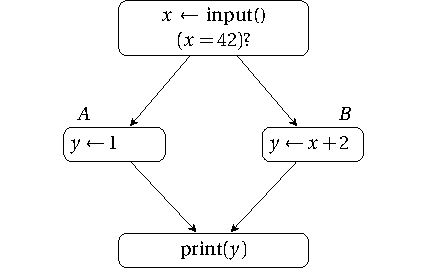
\includegraphics[scale=0.9]{ifthenelse-nonssa.pdf}
\end{minipage}
\bigskip


There is a distinct definition of $y$ in each branch of the \iftt
statement. So multiple definitions of $y$ reach the \texttt{print} statement
at the control-flow merge point. When a compiler transforms this program 
to SSA,
the multiple definitions of $y$ are renamed as $y_1$ and $y_2$. However 
the \texttt{print} statement could use either variable, dependent on the
outcome of the \iftt conditional test. A \phifun introduces
a new variable $y_3$, which takes the value of either $y_1$ or $y_2$.
Thus the SSA version of the program is:
\smallskip

\begin{minipage}{0.4\textwidth}
\begin{equation*}
\begin{array}{l}
x = \texttt{input}();\\
\iftt (x == 42)\\
\\
\thentt\\
\quad    y_1 = 1;\\
\elsett\\
\quad    y_2 = x + 2;\\
\endtt\\
y_3 = \phi(y_1,y_2);\\
\texttt{print}(y_3);\\
\end{array}
\end{equation*}
\end{minipage}
\begin{minipage}{0.4\textwidth}
\strut
\tikzfigure{ifthenelse-ssa}
\end{minipage}
\bigskip


In terms of their position, 
\phifuns\index{\phifun, as multiplexer} are generally placed at control-flow merge points,
i.e., at the heads of basic blocks that have multiple predecessors in
control-flow graphs.
A \phifun at block $b$ has
$n$ parameters if there are $n$ incoming control-flow paths to $b$.
The behavior of the \phifun is to select dynamically
the value of the parameter associated with the actually executed
control-flow path into $b$.
This parameter value is assigned to the fresh variable name,
on the left-hand-side of the \phifun.
Such pseudo-functions are required to maintain the SSA property
of unique variable definitions,
in the presence of branching control flow.
Hence, in the above example, $y_3$ is set to $y_1$ if 
control flows from basic block $A$, and set to $y_2$ if it flows from
basic block $B$.
Notice that the CFG representation here adopts a more expressive syntax for
\phifuns than the standard one, as it associates predecessor basic block labels $B_i$
with corresponding SSA variable names $a_i$, i.e.\
$a_0 = \phi(B_1:a_1, \ldots, B_n:a_n)$.
Throughout this book, basic block labels will be omitted from \phifun
operands when the omission does not cause ambiguity.

It is important to note that, if there are multiple \phifuns\index{\phifun, parallel semantic of}
at the head of a basic block, then these are executed in parallel, 
i.e., simultaneously \textit{not} sequentially.
This distinction becomes important if the target of a \phifun
is the same as the source of another \phifun, perhaps after
optimizations such as copy propagation
(see Chapter~\ref{chapter:constant_propagation_is_easier}).
When \phifuns are eliminated in the SSA destruction phase,
they are sequentialized using conventional 
copy operations,
as described in Chapters~\ref{chapter:classical_construction_algorithm} and~\ref{chapter:alternative_ssa_destruction_algorithm}. This subtlety is particularly important in the context of register allocated code (see Chapter~\ref{chapter:register_allocation}, e.g. Figure~\ref{fig:reg-phifun-seq}).



Strictly speaking, \phifuns are not directly executable in software,
since the dynamic control-flow path leading to the \phifun
is not explicitly encoded as an input to \phifun.
This is tolerable, since \phifuns are generally only 
used during static analysis of the program. They are removed
before any program interpretation or execution takes place.
However, there are various executable extensions of \phifuns, 
such as $\phiif$\index{$\phiif$-function} or $\gamma$\index{$\gamma$-function} functions (see Chapter~\ref{chapter:vsdg}), which take
an extra predicate parameter to replace the implicit
control dependence that dictates the argument the \phifun should select by a condition dependence. Such extensions are useful for program interpretation (see Chapter~\ref{chapter:vsdg}), if-conversion (see~Chapter~\ref{chapter:if_conversion} or), or hardware synthesis (see~\ref{chapter:hardware_compilation}).

%% I would like an example of how to transform a 
%% while loop into SSA, showing how the \phifun
%% must be placed at the loop header. Fabrice doesn't think this
%% example is necessary, but it would be helpful for beginners, I feel...
%% - jsinger
%% Feedback from a reviewer:
%% loop illustrates difference between static and dynamic single/multiple
%% assignments - chris@cs.man.ac.uk

%% example 3. while loop? (iteration)

We present one further example in this section,
to illustrate how a loop control-flow structure appears in SSA.
Here is the non-SSA version of the program and its corresponding control-flow graph SSA version:
\medskip

\begin{minipage}{0.5\textwidth}
\begin{equation*}
\begin{array}{l}
x = 0;\\
y = 0;\\
~\\\\\\\\
\texttt{while} (x < 10) \{\\
~\\\\\\
\quad  y = y + x;\\
\quad  x = x + 1;\\
\}\\
~\\\\
\texttt{print}(y)
\end{array} 
\end{equation*}
\end{minipage}
\begin{minipage}{0.4\textwidth}
\tikzfigure{while}
\end{minipage}
\bigskip

%% In the SSA version below,
%% we abuse conventional C/Java style loop syntax to 
%% enable better program comprehension.
%%   @jsinger - actually, it is legal in GNU C to have
%%   compound statements in a while loop condition...
%%
The SSA code has
% We require initial variable assignments to be
% executed before each evaluation of the loop 
% conditional test.
two \phifuns in the compound loop header
statement that
merge incoming definitions from before the loop
for the first iteration,
and from the loop body for subsequent iterations.
% (Obviously 
% a syntactically correct transformation would rely on
% \texttt{goto} statements to achieve the same effects.)


It is important to outline that SSA should not be confused with (\emph{dynamic}) single assignment (DSA or simply SA) form used in automatic parallelization. \emph{Static} single assignment does not prevent multiple assignments to a variable
during program execution. For instance, in the SSA code fragment above,
variables $y_3$ and $x_3$ in the loop body are 
redefined dynamically with fresh values 
at each loop iteration. 

Full details of the SSA construction algorithm are given in 
Chapter~\ref{chapter:classical_construction_algorithm}. For now, it is sufficient to see that:
\begin{enumerate}
\item A \phifun has been
inserted at the appropriate control-flow merge point where multiple reaching
definitions of the same variable converged in the original program.
\item Integer subscripts have been used to rename
variables~$x$ and~$y$ from the original program.
\end{enumerate}
%%%%%%%%%%%


%%%%%%%%%%%

\section{Comparison with Classical Data Flow Analysis}
\label{sec:vanilla:dfa}
\index{data flow analysis}
% Very simple. Discuss lattice-based data flow analysis.
% Propagating facts around control-flow points in a CFG.
As we will discover further in Chapters~\ref{chapter:ssi} and~\ref{chapter:constant_propagation_is_easier}, one of the major advantages of SSA form concerns data flow analysis.
Data flow analysis collects information about programs
at compile time
in order to make optimizing code transformations.
During actual program execution, information flows between
variables. Static analysis captures
this behaviour by propagating \textit{abstract} information,
or data flow facts,
using an operational representation of the 
program such as the control-flow graph (CFG).
This is the approach used in 
classical data flow analysis.

Often, data flow information can be propagated more efficiently
using a \textit{functional}, or \textit{sparse},
representation of the program such 
as SSA.
% Information that are only related to values can be efficiently 
% propagated using a more functional representation of the program
% along a more sparse evaluation graph (such as SSA).
When a program is translated into SSA form,
variables are renamed at definition points.
For certain data flow problems (e.g.~constant propagation)
this is exactly the set of program points where data flow
facts may change.
Thus it is possible to associate data flow facts directly with 
variable names, rather than
maintaining a vector of data flow facts indexed over all variables,
at each program point.

\begin{figure}[t]%
%\begin{center}
\tikzsubfigures{zero}%
\caption{Example control-flow graph for
  non-zero value analysis, only showing relevant definition statements for
  variables $x$ and $y$.}
\label{fig:part1-vanilla-cfgexample}
%\end{center}
\end{figure}


Figure~\ref{fig:part1-vanilla-cfgexample} illustrates this point through an example of non-zero value analysis\index{data flow analysis, non-zero value}. For each variable in a program, the aim is to determine statically whether
that variable can contain a zero integer value (i.e., null) at runtime. Here $0$ represents the fact that the variable is null, $\nonnull$  the facts that it is non-null, and $\top$\index{top, $\top$} the fact that it is maybe-null. 
%The classical dense data flow analysis approach illustrated in Figure~\ref{fig:part1-vanilla-cfgexample}(a), computes those facts for each variable and each entry and exit of each basic block. The solution of the analysis is expressed as a fixed point solution of a system of data-flow equations. Sparse SSA based data flow analysis, as illustrated in Figure~\ref{fig:part1-vanilla-cfgexample}(b), computes one fact for each SSA variable. As opposed to dense data-flow analysis that has one equation per variable per program point, sparse SSA based data-flow analysis has only one equation per variables definition. The computed fact can be sparsely directly propagated to its uses.
With classical dense data flow analysis\index{data flow analysis, dense} on the CFG in Figure
\ref{fig:part1-vanilla-cfgexample}(a),
we would compute information about variables~$x$ and~$y$ for each of 
the entry and exit points of the six basic-blocks
in the CFG, using suitable data flow equations.
Using sparse SSA-based\index{data flow analysis, sparse} data flow analysis on Figure 
\ref{fig:part1-vanilla-cfgexample}(b),
we compute information about each variable based on a simple
analysis of its definition statement. This gives us six data flow facts,
one for each SSA version of variables $x$ and $y$.

For other data flow problems, properties may 
change at points that are not variable definitions.
These problems can be accommodated in a sparse analysis framework
by inserting additional pseudo-definition functions at appropriate 
points
to induce additional variable renaming. 
See Chapter~\ref{chapter:ssi}
for one such example.
%
However, this example illustrates some key advantages of the SSA-based analysis.
\begin{enumerate}
\item Data flow information
\textit{propagates directly}
from definition statements to uses, via
the def-use\index{def-use chains} links implicit in the SSA naming scheme. 
In contrast, the 
classical data flow framework 
propagates information throughout the program,
including points where the information 
does not change, or is not relevant.
\item The results of the SSA data flow analysis are
\textit{more succinct}.
In the example, there are fewer data flow facts associated with
the sparse (SSA) analysis than with the dense (classical) analysis.
\end{enumerate}

Part~\ref{part:analyses} of this textbook gives a comprehensive treatment of 
some SSA-based data flow analysis.





%%%%%%%%%%%%%%%%

\section{SSA in Context}


% Crib most of this from Kenneth Zadeck. 

% Talk about other program dependence graph
% representations, 

\textbf{Historical Context }
Throughout the 1980s, as optimizing compiler
techology became more mature, various intermediate
representations (IRs) were proposed to encapsulate data
dependence in a way that enabled fast and accurate
data flow analysis.
The motivation behind the design of
such IRs was the exposure of direct links between variable
definitions and uses, known as \textit{def-use chains},
enabling efficient propagation of data-flow information.
% This gives the ability
% to propagate data flow information directly
% from definitions to uses,
% and vice versa.
Example IRs include the program dependence graph \cite{ferrante87program}
and program dependence web \cite{ottenstein90program}.
Chapter~\ref{chapter:vsdg} gives further details on dependence graph
style IRs.

% Talk about early developments at IBM in 1980s.
% Talk about eventual emergence of SSA.

Static single assignment form was one such IR, 
which was developed at IBM Research, and announced publicly
in several research papers in the late 1980s
\cite{rosen88global,alpern88detecting,cytron89efficient}.
SSA rapidly acquired popularity due to its 
intuitive nature and straightforward
construction algorithm.
The SSA property gives a 
standardized shape for variable def-use chains,
which simplifies data flow analysis techniques.

~\\
\textbf{Current Usage }
The majority of current commercial and open-source compilers, including  GCC, Open64, Sun's~HotSpot~JVM, IBM's~Java~Jikes~RVM, Chromium~V8 JavaScript~engine, Mono, and~LLVM,
use SSA as a key intermediate representation for
program analysis.
As optimizations in SSA are fast and powerful, SSA is increasingly used in
just-in-time (JIT) compilers\index{just-in-time compiler, JIT} that operate on a high-level target-independent
program representation such as Java~byte-code, CLI~byte-code (.NET~MSIL), or
LLVM~bitcode.

%% Recent optimizing compiler infrastructures, e.g.~LLVM,  
%% use SSA from the ground up.
%% Other compilers, e.g.~GCC, began
%% development before SSA was well-characterized or
%% widely known.
%% In such cases, SSA support can be back-ported into 
%% the original optimization framework.
%% For instance, GCC uses SSA as of version~4.0.

%% SSA is generally enabled with the \texttt{-O}
%% flag in ahead-of-time compilers (since SSA construction
%% is only required for optimization).
%% Similarly for just-in-time compilers, only the \textit{hot} 
%% methods will be recompiled with SSA-based optimizations.

Initially developed to facilitate the development of high-level
program transformations, SSA form has gained much interest due to its
favorable properties that often
enable the simplification of algorithms and reducuction of computational complexity. 
Today, SSA form is even adopted for the final code generation phase (see Part~\ref{part:machine_code}), i.e., the back-end\index{back-end, compiler}.
Several industrial and academic compilers, static or just-in-time, use SSA in their back-ends, e.g., LLVM, Java~HotSpot, LAO, libFirm, Mono.
Many industrial compilers that use SSA form perform SSA elimination before
register allocation, including  GCC, HotSpot, Jikes, and~LLVM.
Recent research on register allocation\index{register allocation} (see
Chapter~\ref{chapter:register_allocation}) even allows the retention of SSA form until the very end of the code generation process.

~\\
\textbf{SSA for High-Level Languages }
So far, we have presented SSA as a useful feature for 
compiler-based analysis of low-level programs.
It is interesting to note that some high-level languages enforce
the SSA property.
The SISAL language is defined in such a way that
programs automatically have referential transparency, since
multiple assignments are not permitted to variables.
Other languages allow the SSA property to be
applied on a per-variable basis, using special annotations
like
\texttt{final} in Java, or 
\texttt{const} and \texttt{readonly} in C\#.

The main motivation for allowing the programmer to enforce
SSA in an explicit manner in high-level programs is that
\textit{immutability simplifies concurrent programming}.
Read-only data can be shared freely between multiple threads,
without any data dependence problems.
This is becoming an increasingly important issue, with the
trend of multi- and many-core processors.

High-level functional languages\index{functional language} claim
referential transparency as one of the
cornerstones of their programming paradigm.
Thus functional programming supports the SSA property
implicitly.
Chapter~\ref{chapter:semantics} explains the 
dualities between SSA and functional programming.

% However in general,
% it is straightforward to translate a non-SSA program into an SSA
% program. (Links to appropriate chapters here?
% Simple construction / Advanced construction chapters.)



%%%%%%%%%%%%%%%%

\section{About the Rest of this Book}

In this chapter, we have introduced the notion of SSA.
The rest of this book presents various aspects of SSA,
from the pragmatic perspective of compiler engineers and
code analysts. The ultimate goals of this book are:
\begin{enumerate}
\item To demonstrate clearly the \emph{benefits} of SSA-based analysis.
\item To dispell the \emph{fallacies} that prevent people from using SSA.
\end{enumerate}
This section gives pointers to later parts of the book that deal with
specific topics.


\subsection{Benefits of SSA}

% We now conclude by enumerating some of the benefits 
% that it provides.

SSA imposes a strict discipline on variable naming in programs,
so that each variable has a unique definition.
Fresh variable names are introduced at assignment statements,
and control-flow merge points.
This serves to simplify the structure of variable \emph{def-use} 
relationships (see Section~\ref{sec:properties_and_flavours:def-use}) 
and \emph{live ranges} (see Section~\ref{sec:properties_and_flavours:domprop}),
which underpin data flow analysis. Part~\ref{part:analysis} of this book focus
on data flow analysis using SSA. There are three major advantages that SSA enables:
\begin{description}
\item[\textbf{Compile time benefit}]
Certain compiler optimizations can be more efficient
when operating on SSA programs, since
referential transparency means that data flow information
can be associated directly with variables, rather than with variables
at each program point. We have illustrated this simply with the
non-zero value analysis in Section~\ref{sec:vanilla:dfa}.
\item[\textbf{Compiler development benefit}]
Program analyses and transformations can be easier
to express in SSA. This means that compiler engineers
can be more productive, in writing new compiler passes,
and debugging existing passes.
For example, the \textit{dead code elimination} pass
in GCC 4.x, which relies on an underlying SSA-based intermediate
representation, takes only 40\% as many lines of code
as the equivalent pass in GCC 3.x, which does not use SSA.
The SSA version of the pass is simpler, since it
relies on the general-purpose, factored-out, data-flow propagation
engine.
\item[\textbf{Program runtime benefit}]
Conceptually, any analysis and optimization that can be done under SSA form can also be done identically out of SSA form. Because of the compiler development mentioned above, several compiler optimizations show to be more effective
when operating on programs in SSA form. These include the
class of \textit{control-flow insensitive analyses}, e.g.\
\cite{hasti98using}.
\end{description}


\vspace{-2ex}
\subsection{Fallacies about SSA}

Some people believe that SSA is too cumbersome to be an effective
program representation. 
This book aims to convince the reader that
such a concern is
unnecessary,
given the application of suitable techniques.
The table below presents some common myths
about SSA,
and references in this
first part of the book 
containing material to dispell
these myths.

\begin{center}
\small
\begin{tabular}{p{0.38\textwidth}@{\kern.1\textwidth}p{0.5\textwidth}}
\hfil Myth\hfil & \hfil Reference \hfil \\ \hline
SSA greatly increases the number of variables &
Chapter~\ref{chapter:properties_and_flavours} reviews the main varieties of
SSA, some of which introduce far fewer variables\index{variables, number of}
than the original SSA formulation. \\ [1ex]
SSA property is difficult to maintain & 
Chapters~\ref{chapter:classical_construction_algorithm} and~\ref{chapter:repair_maintain_ssa_after_optimization}  discuss simple techniques 
for the repair of SSA invariants that have been
broken by optimization rewrites.\\ [1ex]
SSA destruction\index{SSA destruction} generates many copy\index{copy, insertion} operations & 
Chapters~\ref{chapter:classical_construction_algorithm} and~\ref{chapter:alternative_ssa_destruction_algorithm} present efficient and effective SSA destruction algorithms. \\
\end{tabular}
\end{center}

%%%%%%%%%%%
